\documentclass[conference]{IEEEtran}
\IEEEoverridecommandlockouts

\usepackage{cite}
\usepackage{amsmath,amssymb,amsfonts}
\usepackage{algorithmic}
\usepackage{graphicx}
\usepackage{textcomp}
\usepackage[table]{xcolor}
\usepackage{makecell}
\usepackage{xspace}
\def\BibTeX{{\rm B\kern-.05em{\sc i\kern-.025em b}\kern-.08em
    T\kern-.1667em\lower.7ex\hbox{E}\kern-.125emX}}

\DeclareRobustCommand{\tango}{\textsc{Tango}\xspace}
\DeclareRobustCommand{\dispatcher}{deadline-aware request dispatcher\xspace}
\DeclareRobustCommand{\allocator}{step-time-model-guided token allocator\xspace}
\newcommand{\SJC}[1]{\textcolor{purple}{\textbf{SJC: #1}}}
\DeclareRobustCommand{\redword}[1]{\textcolor{red}{\textbf{#1}}}
\definecolor{FadedFlora}{RGB}{198,239,206}
\newcommand{\CheckmarkBold}{\ensuremath{\boldsymbol{\checkmark}}}
\begin{document}

\title{\tango: \underline{T}emporal-Sp\underline{a}tial Co-Scheduli\underline{ng} for Multi-SL\underline{O} LLM Serving}

% TODO: Add authors and affiliations.
\maketitle
% Show centered page numbers, including on the title page.
\pagestyle{plain}
\thispagestyle{plain}

\begin{abstract}
% Write the abstract.
Online Large Language Model (LLM) serving faces the challenge of delivering high throughput while satisfying heterogeneous latency Service-Level Objectives (SLOs). 
Each request undergoes a prefill phase to produce the first token, followed by a decode phase that generates subsequent tokens, giving rise to two latency metrics: time-to-first-token (TTFT) and time-per-output-token (TPOT).
% However, existing LLM serving systems either ignore heterogeneous SLOs or enforce them only at an aggregate level, resulting in frequent SLO violations under mixed workloads. 
% \SJC{However, existing LLM serving system ignore heterogeneous SLOs of requests, and fail to appropriately schedule the request execution priority and allocte token bugdet to p and d in a batch. (LIKE THAT)}
However, existing LLM serving systems struggle to adapt resource allocation to the varying urgency of requests across prefill and decode phases under heterogeneous SLOs.
We therefore propose \tango, a temporal-spatial co-scheduling framework for Multi-SLO LLM serving. \tango comprises a \dispatcher{} and a \allocator{}. The dispatcher prioritizes requests based on phase-aware SLO deadlines, while the token allocator regulates per-step workloads using predicted execution time. 
Together, they coordinate request ordering and batch composition to improve first-token responsiveness and inter-token timeliness. Experimental results show that \tango improves overall SLO attainment by \redword{58.72\%}, and achieves \redword{1.52}× higher goodput on average than state-of-the-art systems.
\end{abstract}

% \begin{IEEEkeywords}
% % TODO: Add keywords.
% \end{IEEEkeywords}

% !TeX root = ../tango.tex
\section{Introduction}
\label{sec:introduction}

% TODO: Write this section.
Online large language model (LLM) services consolidate requests from multiple applications on shared model instances to improve GPU utilization and reduce serving costs.
These applications impose distinct latency requirements: some requests are sensitive to the delay before the first output token, as in interactive chat, whereas others are sensitive to the delay between consecutive output tokens, as in real-time translation.
These latency requirements are associated with two phases of LLM inference: during \emph{prefill}, the model processes the prompt and generates the first output token; during autoregressive \emph{decode}, it generates subsequent tokens one at a time.
Time to first token (TTFT) measures the delay from request arrival until the first output token is returned, while time per output token (TPOT) measures the average delay per subsequent token.
Online serving systems must therefore maintain high throughput while meeting application-specific TTFT and TPOT service-level objectives (SLOs).


Facing such a scenario, LLM serving aims to improve goodput by satisfying both TTFT and TPOT SLOs for requests with heterogeneous latency requirements.
To support this goal, serving systems combine continuous batching, which dynamically admits new requests into the active batch between iterations, with chunked prefill, which divides long prompts into smaller segments that can be processed alongside decoding requests.
This combination improves GPU utilization and serving efficiency and is adopted by state-of-the-art inference engines such as vLLM and SGLang.


As shown in Fig.~\ref{fig:serving-workflow}, incoming requests first enter the engine's waiting queue.
At each execution step, the scheduler selects waiting requests to run alongside ongoing requests.
It then allocates the step's token budget among these requests to form a batch, specifying the sizes of prefill chunks and the number of decode tokens to include.
The engine then executes the batch, updates request states, and repeats this process for the next step.
We abstract this process into two coupled scheduling dimensions: \emph{temporal scheduling}, which determines request execution priority and admission, and \emph{spatial scheduling}, which determines token allocation within each batch.
These two decisions jointly shape request queueing delay and step duration, thereby affecting TTFT and TPOT.

\begin{figure}[t]
  \centering
  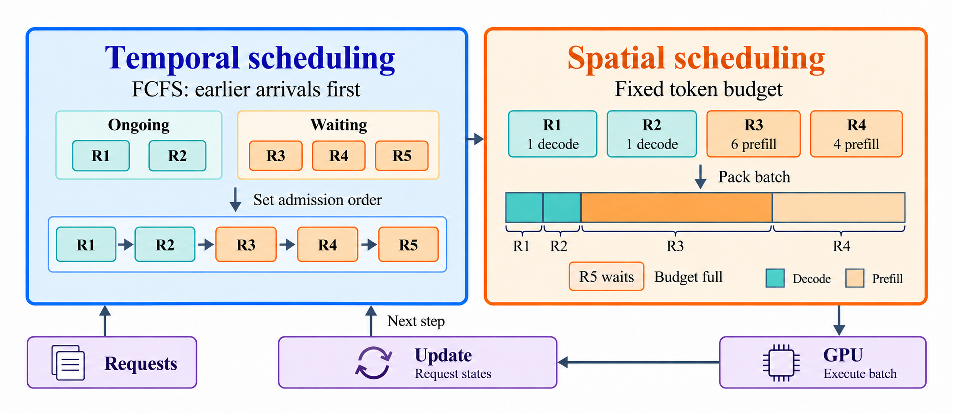
\includegraphics[width=\columnwidth]{figures/introduction/intro.pdf}
  \caption{Temporal and spatial scheduling in LLM serving.}
  \label{fig:serving-workflow}
\end{figure}


Existing throughput-oriented engines commonly use first-come-first-served (FCFS) admission for temporal scheduling and a fixed maximum token budget for spatial scheduling, without adapting these policies to the heterogeneous SLOs of individual requests.
To assess the impact of these policies, we evaluate vLLM's default FCFS scheduler on Qwen3-14B using the mathematical-reasoning workload with heterogeneous TTFT and TPOT requirements.
Among requests with tight TTFT SLOs, only 48.89\% satisfy both SLOs, with TTFT violations accounting for most failures.
For requests with tight TPOT SLOs, joint SLO attainment is similarly low at 12.00\%, with TPOT violations as the main cause.
Across the workload, only 53.48\% of requests satisfy both TTFT and TPOT SLOs.
This low joint attainment highlights the limitations of SLO-unaware scheduling under heterogeneous latency requirements.


First, SLO-unaware temporal scheduling leads to an admission order that does not reflect request urgency.
Under FCFS, a request with a tight TTFT objective can wait behind earlier requests with ample latency slack.
The urgent request may exhaust its TTFT budget in the queue, even though the earlier requests could tolerate being served later.
FCFS therefore misses the opportunity to defer less urgent requests and use their slack to reduce queueing delays for requests with tighter SLOs.


Second, existing spatial scheduling policies allocate tokens under a fixed per-step budget without considering the TPOT requirements of active decode requests.
Because decoding requests must wait for the entire batch to finish before receiving their next tokens, admitting more prefill work can prolong their inter-token delays.
With 2,048 decode tokens fixed, increasing prefill work from zero to 2,048 tokens raises mean step time from 329\,ms to 759\,ms.
Moreover, the same total token count can yield different step times: under a 4,096-token budget, pure-prefill and pure-decode steps take 611\,ms and 683\,ms, respectively, whereas an evenly mixed step takes 759\,ms.
A fixed token budget therefore cannot reliably bound step duration or adapt prefill allocation to the latency tolerance of decoding requests.

Addressing these inefficiencies requires coordinating request-level urgency with batch-level execution time.
First, temporal scheduling involves deciding which waiting requests to admit and which ongoing requests can be deferred under resource contention.
These requests are governed by different active SLOs and have consumed different portions of their latency budgets, so determining their execution order hinges on a consistent comparison of urgency across phases.
Second, spatial scheduling couples the latency requirements of prefill and decode requests through token allocation within a shared batch.
Allocating more tokens to prefill can advance requests with urgent TTFT objectives but also prolong the wait for decoding requests, whereas overly restricting prefill can leave those urgent requests waiting.
Balancing these competing demands requires accurately estimating step time under varying prefill/decode compositions and execution contexts, then using that estimate to guide per-step token allocation.


We therefore propose \tango{}, a multi-SLO LLM serving system that jointly controls temporal request dispatch and spatial token allocation.
\tango{} aims to improve goodput while satisfying heterogeneous TTFT and TPOT requirements.
It comprises a \dispatcher{} and a \allocator{}.
The \dispatcher{} assigns phase-aware deadlines according to each request's active SLO and uses them to guide admission and preemption, prioritizing requests with tighter latency budgets.
The \allocator{} uses a step-time model to predict the execution time of mixed prefill/decode batches and adjusts their prefill token budgets according to the remaining latency slack of decoding requests.


This paper makes three major contributions:
\begin{itemize}
  \item \textbf{Investigating scheduling inefficiencies in multi-SLO LLM serving.}
  The analysis motivates us to account for heterogeneous request urgency and mixed prefill/decode interference through joint control of request dispatch and token allocation.

  \item \textbf{The design of a \dispatcher{} that prioritizes requests across inference phases.}
  By mapping each request's active SLO to a comparable deadline, it guides request admission and preemption, mitigating temporal inefficiency caused by SLO-unaware queueing.

  \item \textbf{The design of a \allocator{} that adapts batch composition to latency constraints.}
  Based on predicted step time, it converts the remaining TPOT slack into a prefill token budget, mitigating mixed prefill/decode interference while preserving progress for requests with tight TTFT requirements.
\end{itemize}


We evaluate \tango{} against vLLM, SOLA, and JITServe using Llama-3.1-8B, Qwen3-14B, and Qwen3-32B under chatbot, mathematical-reasoning, and software-agent workloads.
Compared with state-of-the-art systems, \tango{} improves overall SLO attainment by 58.72\% and achieves $1.52\times$ the goodput on average.

% !TeX root = ../tango.tex
\section{Related Work}
\label{sec:related-work}

\begin{table}[t]
  \renewcommand{\arraystretch}{1.2}
  \setlength{\tabcolsep}{2pt}
  \caption{Scheduling capabilities of representative colocated serving systems.}
  \label{tab:related-work-comparison}
  \centering
  \scriptsize
  \resizebox{\columnwidth}{!}{%
  \begin{tabular}{|l|c|c|c|c|c|}
    \hline
    \textbf{System} &
    \textbf{\makecell{Continuous\\Batching}} &
    \textbf{\makecell{Chunked\\Prefill}} &
    \textbf{\makecell{Heterogeneous\\SLOs}} &
    \textbf{\makecell{Request-Specific\\SLO Prioritization}} &
    \textbf{\makecell{Deadline-Aware\\Token Allocation}} \\
    \hline
    \bfseries vLLM & \cellcolor{FadedFlora}\CheckmarkBold & \cellcolor{FadedFlora}\CheckmarkBold & -- & -- & -- \\
    \hline
    \bfseries Sarathi-Serve & \cellcolor{FadedFlora}\CheckmarkBold & \cellcolor{FadedFlora}\CheckmarkBold & -- & -- & -- \\
    \hline
    \bfseries SOLA & \cellcolor{FadedFlora}\CheckmarkBold & \cellcolor{FadedFlora}\CheckmarkBold & -- & -- & -- \\
    \hline
    \bfseries JITServe & \cellcolor{FadedFlora}\CheckmarkBold & \cellcolor{FadedFlora}\CheckmarkBold & \cellcolor{FadedFlora}\CheckmarkBold & \cellcolor{FadedFlora}\CheckmarkBold & -- \\
    \hline
    \bfseries \tango{} & \cellcolor{FadedFlora}\CheckmarkBold & \cellcolor{FadedFlora}\CheckmarkBold & \cellcolor{FadedFlora}\CheckmarkBold & \cellcolor{FadedFlora}\CheckmarkBold & \cellcolor{FadedFlora}\CheckmarkBold \\
    \hline
  \end{tabular}%
  }
  \vspace{-3mm}
\end{table}

\textbf{SLO-Agnostic LLM Serving.}
Existing LLM serving systems improved throughput and latency through efficient batching and memory management.
Orca introduced iteration-level scheduling, which allowed requests to enter and leave a batch between decoding iterations.
vLLM introduced PagedAttention to reduce KV-cache fragmentation and support flexible memory sharing.
SGLang exploited prefix reuse through RadixAttention and optimized the execution of structured language model programs.
However, these works optimized batching and memory efficiency without explicitly accounting for each request's TTFT and TPOT objectives in scheduling.

\textbf{SLO-Aware Temporal Request Scheduling.}
SLO-aware temporal schedulers used latency requirements to decide which requests received service.
SOLA adjusted request priorities and iteration workloads based on request progress and system state to improve SLO attainment for both TTFT and TPOT.
However, its shared TTFT and average-TPOT targets could not directly express heterogeneous request SLOs, and its token budgeting did not explicitly enforce individual next-token deadlines.
For requests with heterogeneous SLOs, JITServe progressively refined estimates of output lengths and request dependencies to prioritize requests by their expected goodput and the serving bandwidth required to meet their SLOs, and grouped requests with similar input lengths to improve batching efficiency.
However, this request-specific SLO prioritization operated at the inter-request level without explicitly accounting for intra-batch prefill--decode contention.

\textbf{Spatial Prefill--Decode Scheduling.}
Existing approaches mitigated prefill--decode interference through resource separation or control of batch workloads.
DistServe placed prefill and decode on separate GPUs to eliminate interference and independently optimized their resource allocation and parallelism to meet TTFT and TPOT requirements.
Sarathi-Serve instead split long prompts into smaller prefill chunks and batched them with ongoing decode requests under a fixed token budget to reduce interference.
However, these approaches relied on phase-level resource partitioning or fixed token budgets, limiting their ability to accommodate heterogeneous TTFT and TPOT requirements.


Table~\ref{tab:related-work-comparison} compares \tango{} with representative works.

% !TeX root = ../tango.tex
\section{Background and Motivation}
\label{sec:background-and-motivation}

\subsection{Multi-SLO LLM Serving}
\label{sec:multi-slo-llm-serving}

\textbf{LLM Inference and Latency SLOs.}
An online LLM serving engine processes each request in two phases.
During \emph{prefill}, the engine processes all prompt tokens in parallel, constructs their key--value (KV) caches, and produces the first output token.
During \emph{decode}, it reuses the KV caches and autoregressively generates subsequent output tokens, typically one token per request in each iteration.
The two phases expose different forms of latency and corresponding service-level objectives (SLOs): a request must first wait for its prompt to be processed, and must then make timely progress over a sequence of decoding iterations.
Let request $r_i$ arrive at time $a_i$ and generate $n_i$ output tokens, where $t_{i,j}$ denotes the time at which its $j$-th output token is returned.
Its time to first token (TTFT) and time per output token (TPOT) are defined as
\begin{equation}
  \begin{aligned}
    \mathrm{TTFT}_i &= t_{i,1} - a_i, \\
    \mathrm{TPOT}_i &= \frac{1}{n_i-1}
      \sum_{j=2}^{n_i}\left(t_{i,j}-t_{i,j-1}\right),
      \quad n_i > 1.
  \end{aligned}
  \label{eq:latency-metrics}
\end{equation}
TTFT captures the queuing and prefill delay before a response begins, whereas TPOT captures the average interval between consecutive tokens after generation starts.
Each request is associated with a pair of latency objectives, denoted by $S_i^{\mathrm{TTFT}}$ and $S_i^{\mathrm{TPOT}}$.
Request $r_i$ satisfies its SLOs only if
$\mathrm{TTFT}_i \leq S_i^{\mathrm{TTFT}}$ and
$\mathrm{TPOT}_i \leq S_i^{\mathrm{TPOT}}$.
In this work, \emph{Multi-SLO} refers both to these phase-specific objectives and to their heterogeneous values across requests and applications.
Accordingly, serving efficiency is measured by goodput---the rate of requests that satisfy both objectives---rather than by raw request or token throughput alone.

\textbf{Continuous Batching and Chunked Prefill.}
In static batching, a newly arrived request cannot join an executing batch until every request in that batch finishes, which wastes GPU capacity as requests complete at different times.
Continuous batching instead updates the active batch at iteration boundaries.
After each iteration, completed requests leave, unfinished decode requests remain active, and waiting requests can be admitted into the released capacity.
The batch composition can thus evolve throughout generation, improving GPU utilization while allowing the scheduler to reconsider which requests should run at every step.

A prefill request may contain hundreds or thousands of prompt tokens, whereas an active decode request contributes only its next token to an iteration.
Scheduling an entire prompt at once can therefore produce a long iteration and delay token generation for the decode requests in the same batch.
Chunked prefill divides the prompt into smaller chunks that may be processed over multiple iterations.
This enables prefill chunks and decode tokens to be colocated in one batch, while exposing the prefill chunk size as a controllable scheduling variable.
Specifically, let $\mathcal{P}_k$ and $\mathcal{D}_k$ denote the prefill and decode requests selected in step $k$, respectively, and let $c_{i,k}$ be the number of prompt tokens allocated to prefill request $r_i$.
The number of tokens scheduled in this step is
\begin{equation}
  T_k = \sum_{r_i \in \mathcal{P}_k} c_{i,k}
        + \lvert\mathcal{D}_k\rvert,
  \qquad T_k \leq B_{\max},
  \label{eq:step-token-budget}
\end{equation}
where each decode request contributes one token and $B_{\max}$ is the engine's maximum per-step token budget.
The resulting queueing delay and intervals between decoding iterations determine whether each request meets its TTFT and TPOT objectives.

\subsection{Multi-SLO Traces for Investigations}
\label{subsec:motivation-trace}

We construct three representative LLM inference workloads covering conversational assistance, mathematical reasoning, and software-engineering agents.

\textbf{Chatbots.}
We construct chatbot requests from LMSYS-Chat-1M, which contains one million real-world conversations collected from interactions with 25 LLMs.
The token length of each recorded response determines its target output length.

\textbf{Mathematical Reasoning.}
We use all 8,792 questions from the training and test splits of GSM8K.
Each word problem serves as the input prompt, while the token length of its reference solution determines the target output length.

\textbf{Software Agents.}
We use the software-engineering subset of AgentWorldBench and retain one request from each of 99 distinct trajectories.
For each request, we generate 1,024 variants by prepending a distinct synthetic prefix while preserving the original agent action and target environment observation.

From the three request pools, we randomly sample 10,000 chatbot, 8,000 mathematical-reasoning, and 4,000 software-agent requests to form the replay traces.


\textbf{Arrivals and SLOs.}
We associate requests in order with timestamps from failure-free entries in BurstGPT and replay each workload according to these timestamps, thereby preserving the trace's temporal arrival pattern.
For each workload, we first determine the sending rate $\lambda_{90}$ at which vLLM achieves a 90\% SLO attainment rate.
We then set the sending rate to $1.2\lambda_{90}$ to emulate a workload under pressure.

For each request, we execute it alone on an otherwise idle vLLM deployment and record its measured TTFT and TPOT.
These isolated measurements serve as request-specific latency baselines.
We derive the two SLOs of request $r_i$ as
\begin{equation}
  \begin{aligned}
    S_i^{\mathrm{TTFT}} &= c_i^{\mathrm{TTFT}}
      \widehat{\mathrm{TTFT}}_i, \\
    S_i^{\mathrm{TPOT}} &= c_i^{\mathrm{TPOT}}
      \widehat{\mathrm{TPOT}}_i,
  \end{aligned}
  \label{eq:slo-generation}
\end{equation}
where $\widehat{\mathrm{TTFT}}_i$ and $\widehat{\mathrm{TPOT}}_i$ are the isolated-run measurements, and $c_i^{\mathrm{TTFT}}$ and $c_i^{\mathrm{TPOT}}$ are the coefficients assigned to the request's SLO class.
Using a fixed random seed, we assign requests equally among four SLO classes: TTFT-prioritized, TPOT-prioritized, balanced, and relaxed.
For Qwen3-14B, the TTFT/TPOT coefficient pairs for these four classes are $(20, 2.5)$, $(50, 1.5)$, $(25, 2)$, and $(50, 3)$, respectively.
All compared systems use the same request sequence, arrival schedule, and SLO targets under each experimental condition.



\begin{table}[t]
  \renewcommand{\arraystretch}{1.05}
  \setlength{\tabcolsep}{3pt}
  \caption{Experimental setup.}
  \label{tab:motivation-setup}
  \centering
  \scriptsize
  \resizebox{\columnwidth}{!}{%
  \begin{tabular}{c|c}
    \hline
    & \textbf{Specifications} \\
    \hline
    \textbf{Hardware} & \makecell[c]{$2\times$ Intel Xeon Gold 6530 CPUs, 64 physical cores \\
      128 logical threads, 377.6 GiB host RAM (OS-reported) \\
      $4\times$ RTX 6000 Ada GPUs (48 GB each); $2\times$ GPUs used per run} \\
    \hline
    \textbf{Software} & \makecell[c]{Qwen/Qwen3-14B (TP${}={}$2); vLLM 0.17.0 \\
      PyTorch 2.10.0+cu128; CUDA 12.8; driver 570.124.06 \\
      LMSYS-Chat-1M, GSM8K, AgentWorldBench-SWE, BurstGPT} \\
    \hline
  \end{tabular}%
  }
\end{table}

\subsection{Low Multi-SLO Serving Performance}
\label{subsec:low-multi-slo-performance}

\begin{table}[t]
  \centering
  \caption{SLO attainment of vLLM on the math workload.}
  \label{tab:fcfs-multi-slo-attainment}
  \scriptsize
  \setlength{\tabcolsep}{3pt}
  \renewcommand{\arraystretch}{1.10}
  \begin{tabular}{lccc}
    \hline
    \textbf{SLO Class} &
    \textbf{TTFT (\%)} &
    \textbf{TPOT (\%)} &
    \textbf{Joint (\%)} \\
    \hline
    Overall          & \textbf{75.80} & \textbf{77.68} & \textbf{53.48} \\
    TTFT-prioritized & 48.89 & 100.00 & 48.89 \\
    TPOT-prioritized & 100.00 & 12.00 & 12.00 \\
    Balanced         & 57.39 & 100.00 & 57.39 \\
    Relaxed          & 100.00 & 100.00 & 100.00 \\
    \hline
  \end{tabular}
\end{table}

We use vLLM's default FCFS scheduler as a representative serving baseline.
It supports continuous batching and chunked prefill, but schedules requests without differentiating their TTFT and TPOT objectives.
We run Qwen3-14B with TP${}={}$2 on two GPUs using the configuration in Table~\ref{tab:motivation-setup}.
We use the math workload as a representative case and replay it at its stress load of $1.2\lambda_{90}$.

Table~\ref{tab:fcfs-multi-slo-attainment} summarizes the SLO attainment rates for the math workload.
Under FCFS, the overall TTFT and TPOT attainment rates are 75.80\% and 77.68\%, respectively, but only 53.48\% of requests satisfy both objectives.
The gap between individual and joint attainment shows that satisfying either latency objective alone does not provide effective Multi-SLO service.

The class-level results further reveal distinct failure modes.
TTFT-prioritized requests achieve 48.89\% TTFT attainment and 100.00\% TPOT attainment, whereas TPOT-prioritized requests achieve 100.00\% and 12.00\%, respectively.
Balanced and relaxed requests attain both objectives for 57.39\% and 100.00\% of their requests, respectively.
The contrasting class-level results indicate that the low joint attainment cannot be attributed to a single global latency bottleneck.

Together, these observations expose a mismatch between throughput-oriented scheduling and request-specific latency objectives.
FCFS fixes the service order according to request arrival and does not account for the remaining TTFT or TPOT slack when admitting prefill chunks or advancing decode requests.
Consequently, a scheduling decision that preserves prompt responsiveness may disrupt token delivery, while one that protects decode progress may increase the waiting time of queued prefills.
The serving engine can therefore retain sufficient capacity to satisfy 100.00\% of the relaxed requests, yet fail to direct that capacity toward the phase-specific objectives of other requests.
These observations motivate a closer examination of how request ordering and per-step token allocation jointly affect Multi-SLO attainment.

\subsection{Diving into Underlying Reasons}
\label{subsec:motivation-underlying-reasons}

Our investigation identifies two complementary causes of the low Multi-SLO attainment: 1) FCFS distributes queueing delay without considering request-specific TTFT urgency, and 2) a fixed token budget does not provide a reliable latency bound for steps that mix prefill and decode tokens.

\begin{figure}[!t]
  \centering
  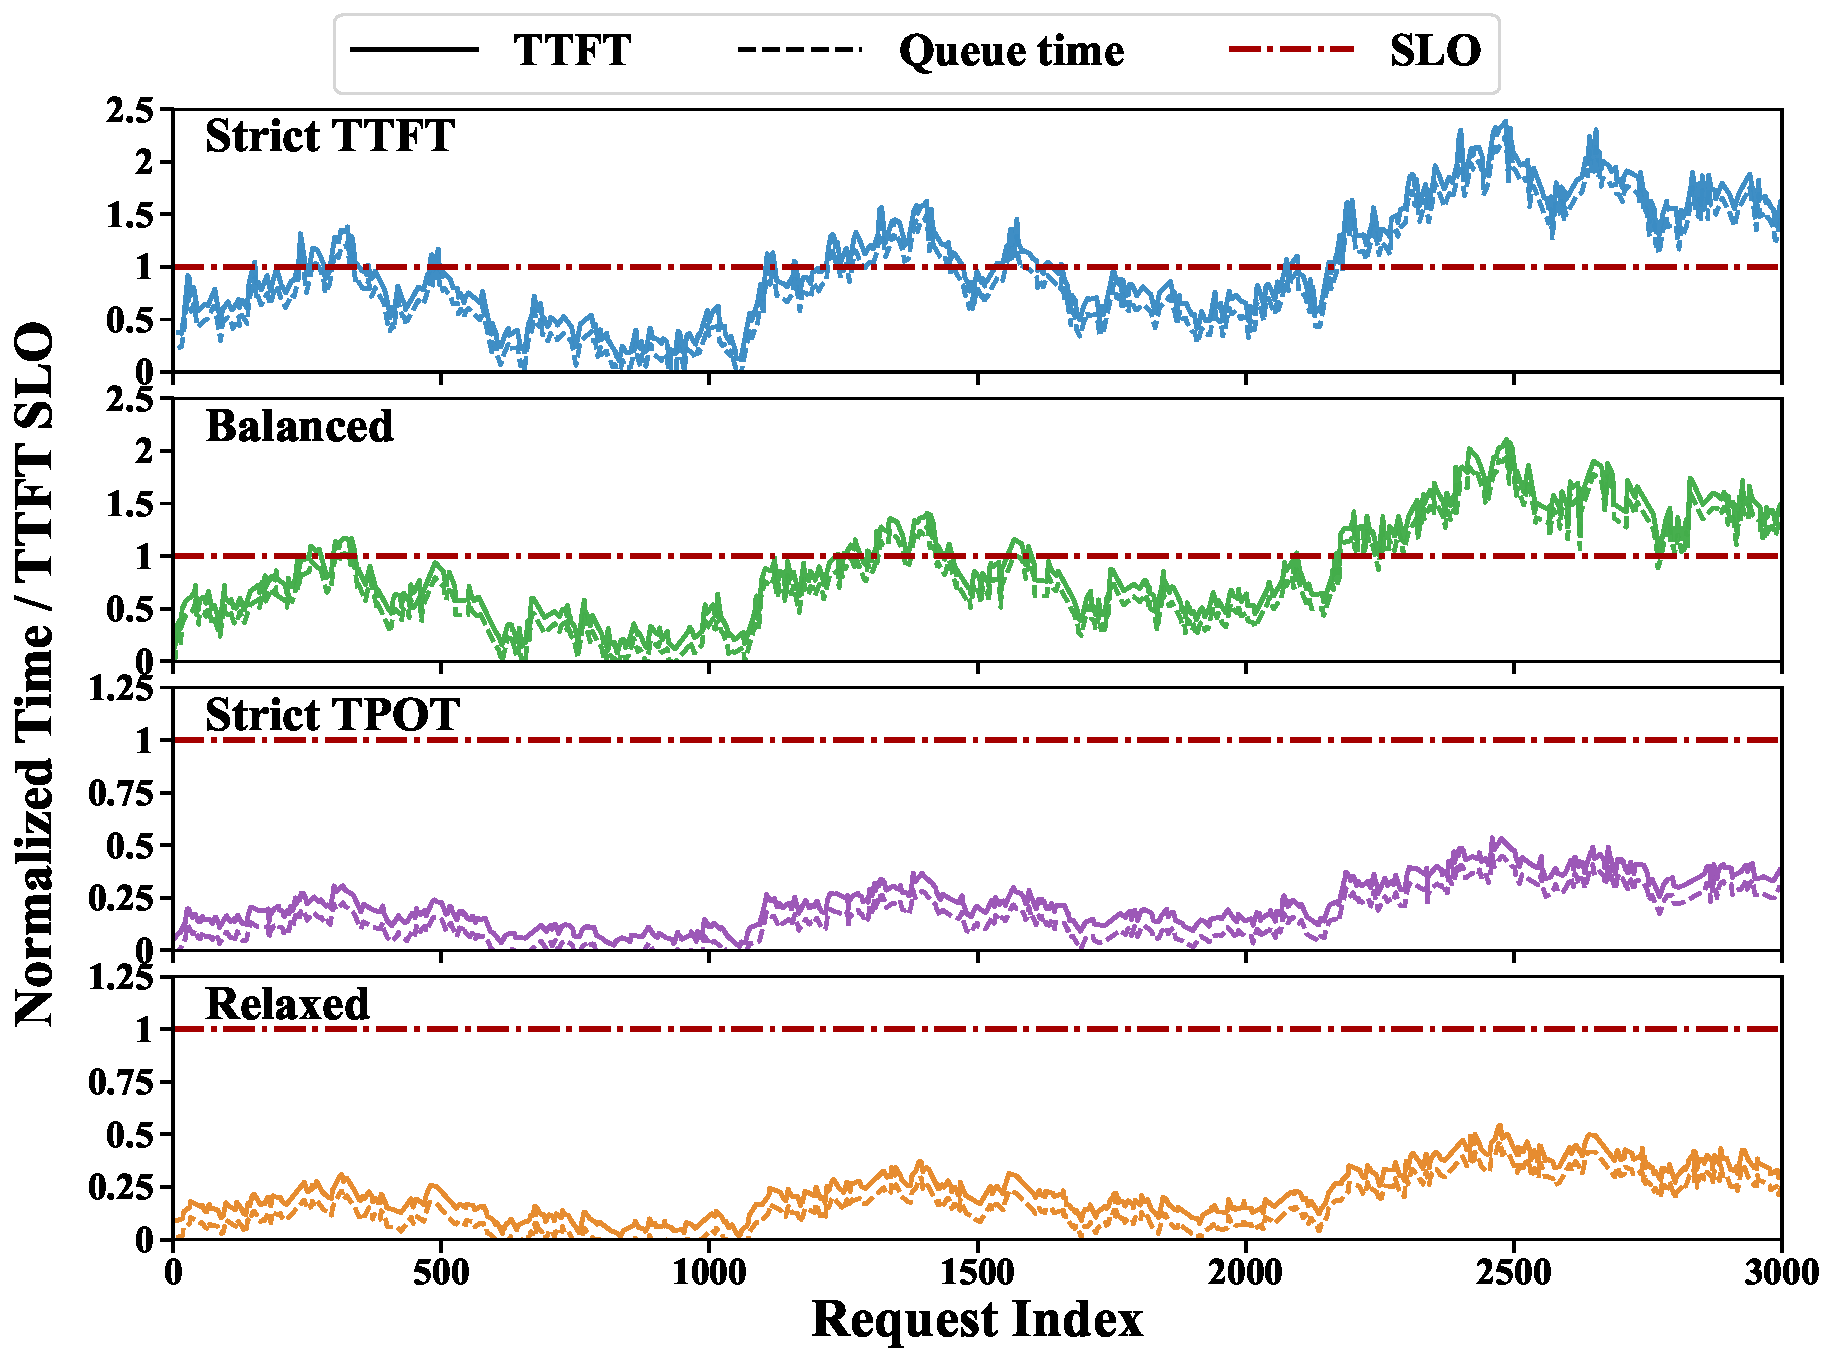
\includegraphics[width=0.94\columnwidth]{figures/background-and-motivation/moti_queue_slo}
  \caption{Normalized TTFT and queueing time under FCFS.}
  \label{fig:temporal-slo-ratio}
\end{figure}

\noindent\textbf{1) SLO-unaware temporal scheduling.}
The first-token latency of request $r_i$ can be decomposed as
\begin{equation}
  \mathrm{TTFT}_i = W_i^{\mathrm{queue}} + L_i^{\mathrm{prefill}},
  \label{eq:ttft-decomposition}
\end{equation}
where $W_i^{\mathrm{queue}}$ is the delay from arrival until the request is first admitted for prefill, and $L_i^{\mathrm{prefill}}$ is the remaining latency until its first token is produced.
For a chunked prefill, $L_i^{\mathrm{prefill}}$ includes the execution and intervening scheduling delays of all prompt chunks after admission.

Fig.~\ref{fig:temporal-slo-ratio} plots TTFT and queueing time for the first 3,001 math requests, normalized by each request's TTFT SLO.
Solid and dashed lines denote TTFT and queueing time, respectively; the dash-dotted line marks the SLO boundary.
The Strict TTFT and Strict TPOT panels correspond to the TTFT-prioritized and TPOT-prioritized classes, respectively.
The normalized queueing-time curve closely follows the TTFT curve in all four SLO classes, indicating that queueing dominates the first-token latency.
For TTFT-prioritized and balanced requests, the queueing delay frequently consumes most, or even all, of the TTFT budget before prefill completes.
TPOT-prioritized and relaxed requests remain below the boundary because their looser TTFT objectives provide substantially more slack.
The resulting TTFT violations therefore arise primarily from how waiting time is distributed among requests, rather than from a uniform shortage of prefill compute capacity.

FCFS creates this imbalance because it admits requests according to arrival order, regardless of their remaining TTFT slack.
A TTFT-prioritized request may wait behind earlier requests whose looser objectives could tolerate additional delay; the urgent request exhausts its latency budget in the queue while those ahead of it still finish within their SLOs.
The temporal scheduling problem is thus to determine \emph{which request} should receive prefill service first.
Accounting for the remaining TTFT slack can redistribute queueing delay toward requests that can tolerate it, without changing the total amount of prefill work.

\begin{figure}[!t]
  \centering
  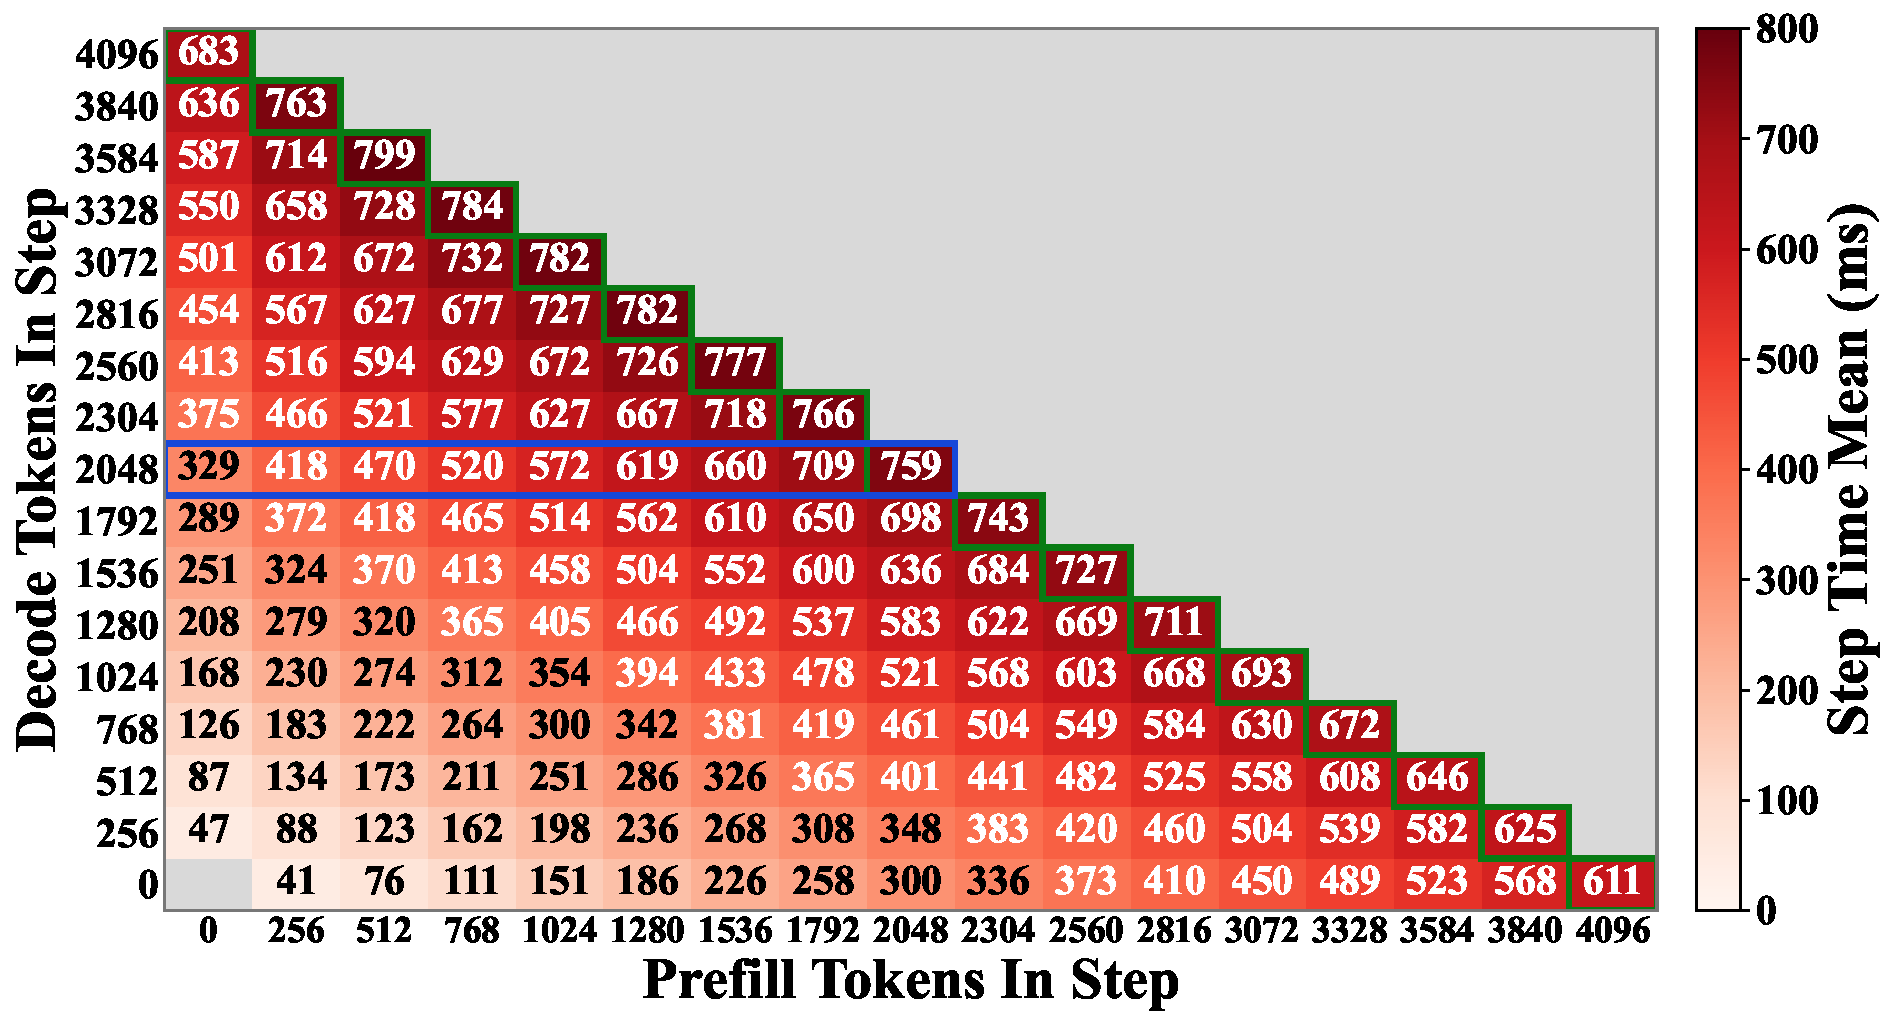
\includegraphics[width=\columnwidth]{figures/background-and-motivation/moti_token_heatmap}
  \caption{Mean step time with different prefill and decode token counts.}
  \label{fig:spatial-pd-grid}
\end{figure}

\noindent\textbf{2) Workload-unaware spatial scheduling.}
The second failure mode arises after requests enter the running batch.
For an active decode request, the interval before its next token is determined by the duration of the engine step in which that token is scheduled.
Reordering waiting requests alone cannot protect TPOT because a decode token may still share a step with a large prefill chunk.

To quantify this interference, we vary the numbers of prefill tokens $p$ and decode tokens $d$ scheduled in the same step and measure the mean step time.
Each configuration is measured on Qwen3-14B with TP${}={}$2 over 50 timed steps (5 rounds $\times$ 10 measurements); gray cells exceed the maximum per-step token budget.
As highlighted by the blue outline in Fig.~\ref{fig:spatial-pd-grid}, when $d=2{,}048$, increasing $p$ from 0 to 2,048 increases the mean step time from 329\,ms to 759\,ms.
Every active decode request must wait for the longer step to complete before receiving its next token, directly increasing its TPOT.

More importantly, the total token count alone does not determine step time.
Along the green boundary where $p+d=4{,}096$, the pure-prefill and pure-decode configurations take 611\,ms and 683\,ms, respectively, while mixed configurations reach up to 799\,ms.
Thus, the same total token budget produces about a $1.3\times$ difference in latency.
This nonlinearity reflects the distinct execution characteristics of compute-intensive prefill and memory-intensive decode, together with their interference when colocated in one iteration.
Consequently, enforcing only $p+d\leq B_{\max}$ bounds the amount of scheduled work but cannot reliably bound the wall-clock latency experienced by active decode requests.

The spatial scheduling problem is therefore to determine \emph{how many prefill tokens} can safely share the next step with the current decode workload.
This requires an estimate of mixed-step latency and a mechanism that converts the remaining TPOT slack of active requests into a safe prefill allocation.
Temporal request ordering and spatial token allocation address different failure modes: optimizing either dimension alone leaves the other source of SLO violations unresolved.
These observations motivate their joint design in \tango{}.

% !TeX root = ../tango.tex
\section{TANGO Methodology}
\label{sec:tango-methodology}

Fig.~\ref{fig:tango-overview} shows the design overview of \tango{}, which comprises a \dispatcher{} and a \allocator{}.
At each iteration boundary, the two components coordinate request execution priority and per-step token allocation according to heterogeneous TTFT and TPOT SLOs.
They take each request's SLOs, inference phase, and execution progress as input and produce a mixed batch of prefill chunks and decode tokens.

\begin{figure}[t]
  \centering
  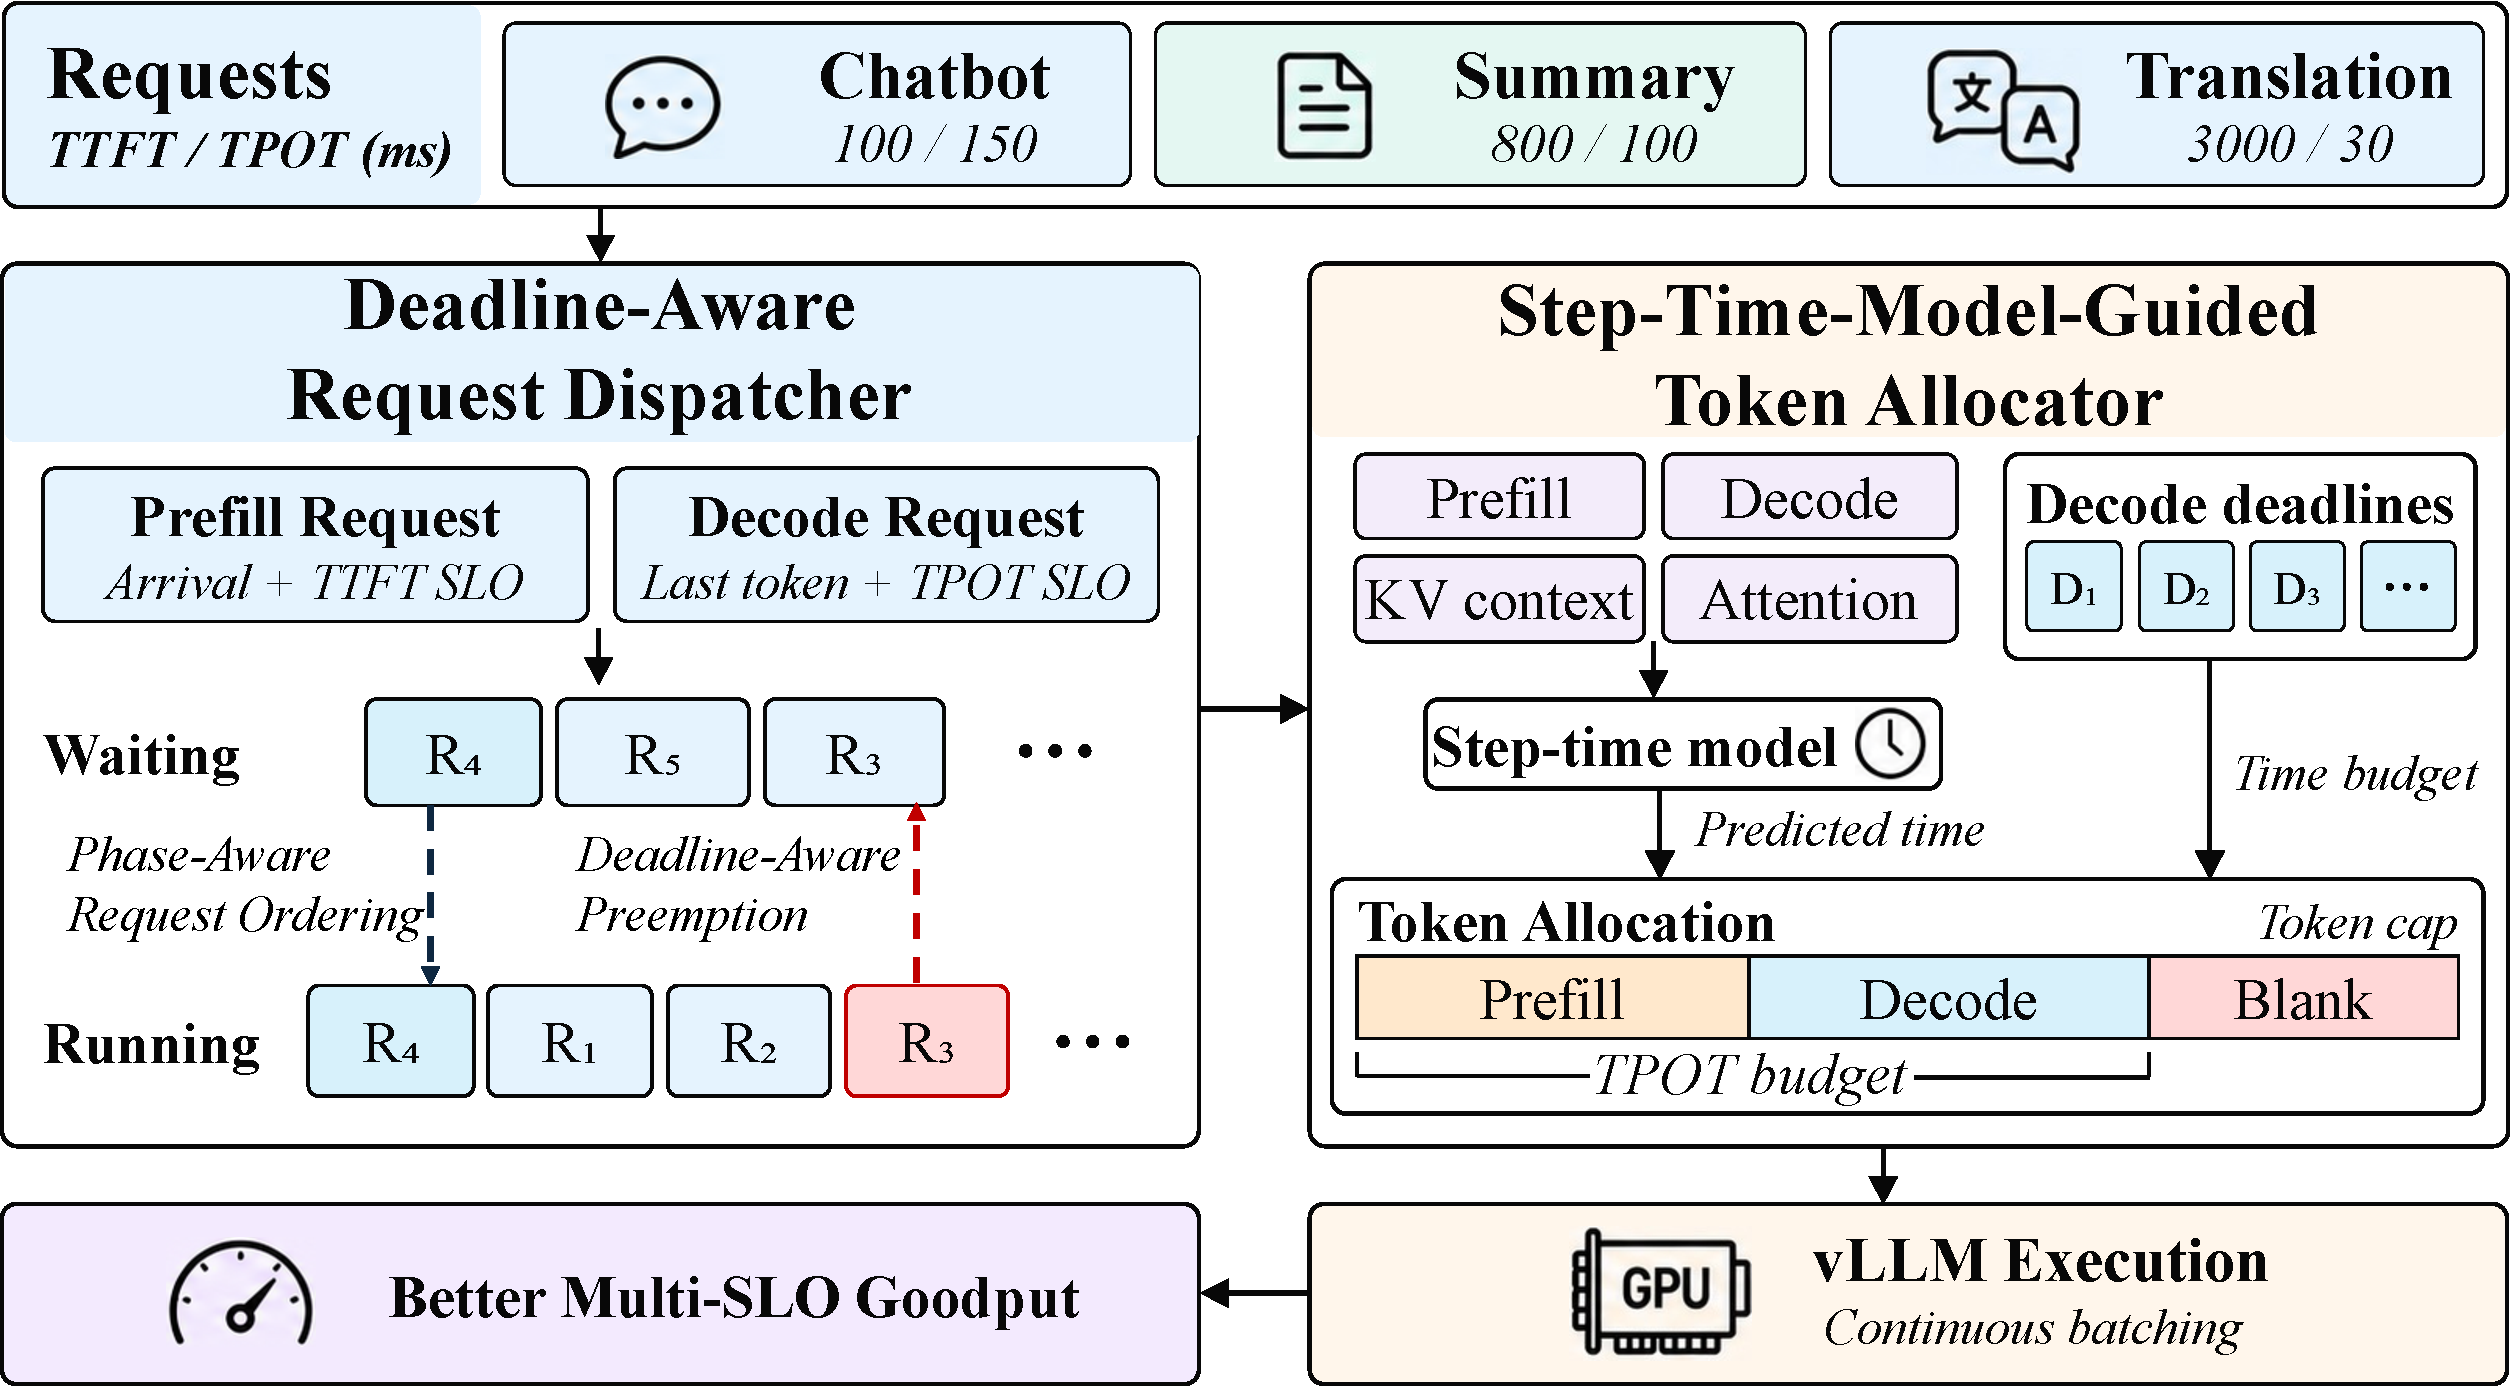
\includegraphics[width=\columnwidth]{figures/tango-methodology/overview}
  \caption{Design overview of \tango{}.}
  \label{fig:tango-overview}
\end{figure}

The temporal scheduling challenge is to compare request urgency across inference phases.
A request with an unfinished prefill must produce its first token within its TTFT budget, whereas a decoding request must sustain token-generation progress within its TPOT budget.
The dispatcher maps these phase-specific requirements to comparable deadlines and updates request priorities as inference progresses.
These priorities guide the admission of waiting requests and the preemption of less urgent ongoing requests under resource contention (Section~\ref{sec:deadline-aware-request-dispatcher}).

The spatial scheduling challenge is to advance urgent prefills while limiting their interference with decoding requests.
As shown in Section~\ref{subsec:motivation-underlying-reasons}, the total token count alone cannot reliably determine mixed-step execution time.
The allocator therefore uses a step-time model to predict the duration of candidate batches from their prefill/decode composition and context-dependent attention work.
It converts the remaining deadline slack of selected decode requests into a prefill token budget and distributes that budget according to the dispatcher's priorities (Section~\ref{sec:step-time-model-guided-token-allocator}).

Specifically, \tango{} operates as follows.
First, the scheduler collects the running requests' execution state, and the allocator derives a prefill token budget using the step-time model.
Second, the dispatcher orders waiting requests by their phase-aware deadlines for admission alongside ongoing requests.
If a waiting request cannot obtain KV-cache blocks, the dispatcher considers preempting the running request with the latest deadline, but proceeds only when the waiting request has an earlier deadline.
The allocator applies the remaining token and time budgets to the prefill chunks of ongoing and newly admitted requests.
Finally, the engine executes the resulting batch and returns token timestamps and request progress to update the next scheduling decision.
Unfinished requests remain eligible for reconsideration at the next iteration boundary.

The example in Fig.~\ref{fig:tango-overview} illustrates how the two components cooperate.
An urgent waiting request $r_4$ receives earlier admission, while a less urgent ongoing request can be preempted to release capacity.
The allocator then determines how much of the admitted request's prompt can share a step with the active decode workload.
When the decode requests have little remaining deadline slack, it limits the prefill chunk size and leaves the remaining prompt tokens for subsequent steps, even if the engine's maximum token capacity has not been exhausted.
Thus, request urgency determines the service order, while predicted step time determines how much work can execute in that order.

% !TeX root = ../tango.tex
\subsection{\dispatcher{}}
\label{sec:deadline-aware-request-dispatcher}

% TODO: Write this section.

% !TeX root = ../tango.tex
\subsection{\allocator{}}
\label{sec:step-time-model-guided-token-allocator}

% 第1段：结合执行流程图介绍 allocator 如何用预测步耗时将 decode 时间预算转为 prefill 配额；交代模型、联合预算和执行流程的结构。
Fig.~\ref{fig:token-allocator-workflow} shows how the allocator determines the amount of prefill work that can share an engine step with the active decode workload.
Its key idea is to translate the remaining next-token time budget into a prefill token allocation using a fitted step-time model.
In this section, we first introduce the model, then explain how heterogeneous TTFT and TPOT objectives guide budgeting, and finally describe the allocation workflow.

% 图注：简述 allocator 执行流程；虚线含义与符号说明见正文。
\begin{figure}[t]
  \centering
  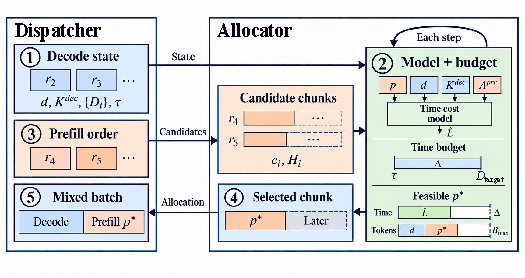
\includegraphics[width=\columnwidth]{figures/tango-methodology/token-allocator-workflow.pdf}
  \caption{Execution workflow of the \allocator{}.}
  \label{fig:token-allocator-workflow}
\end{figure}

\subsubsection{Step-Time Modeling}
\label{subsec:step-time-modeling}

% 第2段提纲：从固定 token 总数不能约束混合步延迟的问题出发，定义四个工作量特征并给出模型；沿用已有 p/d 及 batch 记号，避免与 request deadline D_i 混淆。
As analyzed in Section~\ref{subsec:motivation-underlying-reasons}, batches with the same total token count can have substantially different execution times.
The predictor must therefore account for both batch composition and context-dependent attention work.
Let $p$ and $d$ denote the numbers of prefill and decode tokens, respectively, $K^{\mathrm{dec}}$ the sum of context lengths accessed by decode requests, and $A^{\mathrm{pre}}$ the effective attention work of prefill chunks.
These four inputs feed the time cost model in Fig.~\ref{fig:token-allocator-workflow}, which estimates the step duration as
\begin{equation}
  \widehat{L}\!\left(p,d,K^{\mathrm{dec}},A^{\mathrm{pre}}\right)
  = \alpha + \beta p + \gamma d
    + \delta K^{\mathrm{dec}} + \epsilon A^{\mathrm{pre}}.
  \label{eq:step-time-model}
\end{equation}

% 第3段提纲：逐项解释模型与主要执行成本的对应关系，说明这些项是拟合得到的近似，而非每种操作的精确计时。
Each term approximates a different source of execution cost.
The intercept $\alpha$ captures the fixed runtime cost of a step, while $\beta p$ and $\gamma d$ capture the token-dependent costs of prefill and decode computation.
The term $\delta K^{\mathrm{dec}}$ accounts for decode attention's KV-cache reads, which grow with the total history accessed by decode tokens.
Finally, $\epsilon A^{\mathrm{pre}}$ accounts for the attention computation performed by prefill chunks.

% 第4段提纲：给出 chunked prefill attention 工作量的构造；解释历史 prefix 与 chunk 长度共同决定成本，避免将多个请求的 token 总数直接平方；说明部署配置相关的离线拟合与运行时求值。
For chunked prefill, the attention work depends on both the new chunk and its existing prefix.
Let $H_{i,k}$ be the already-computed context length available to request $r_i$ before step $k$.
Using the chunk sizes $c_{i,k}$ defined in Eq.~\ref{eq:step-token-budget}, we approximate the attention work as
\begin{equation}
  A_k^{\mathrm{pre}} =
  \sum_{r_i\in\mathcal{P}_k}
    c_{i,k}\left(H_{i,k}+\frac{c_{i,k}}{2}\right).
  \label{eq:prefill-attention-work}
\end{equation}
A single fresh prefill thus contributes approximately $p^2/2$, whereas a chunk following a long prefix incurs additional work proportional to that prefix length.
Consequently, equal-sized chunks can consume different amounts of the step-time budget.
The coefficients are fitted from profiled engine steps for the deployed model and hardware configuration.
At runtime, prediction requires only these four workload statistics and a few arithmetic operations.

\subsubsection{Joint TTFT/TPOT Budgeting}
\label{subsec:joint-slo-budgeting}

% 第5段提纲：先固定当前 running decode 工作量，再从 TPOT deadline 集合选取约束本轮步耗时的 deadline；说明基准分位数控制对紧迫 decode 请求的保护程度。
At the beginning of step $k$, the allocator summarizes the active decode workload as $d_k=\lvert\mathcal{D}_k\rvert$ and $K_k^{\mathrm{dec}}=\sum_{r_i\in\mathcal{D}_k}H_{i,k}$.
Each decode request contributes its next-token deadline $D_i$ from Eq.~\ref{eq:phase-aware-deadline}.
The allocator selects a binding deadline from this set using a configurable percentile $\rho_0\in[0,1]$.
With $\rho_0=0$, the earliest deadline bounds the predicted step duration; a larger percentile selects a later deadline and permits more prefill work.

% 第6段提纲：解释单纯保护 TPOT 可能挤压紧迫 TTFT；用归一化剩余时间比较两类目标，按毕业论文保留自适应分位数策略，明确放宽较早 decode deadline 是联合调度中的取舍。
% 实现核对：毕业论文仅说明 TTFT 更紧迫时将分位数向 1 调整；基准值及具体调整映射待确认，此处不假设数值或额外公式。
A fixed decode percentile can leave urgent prefills with insufficient service even when increasing prefill work would improve first-token responsiveness.
To account for this tradeoff, the allocator compares the remaining fractions of the two latency budgets.
At scheduling time $\tau_k$, these fractions are
\begin{equation}
  \begin{aligned}
    u_{i,k}^{\mathrm{TTFT}} &=\frac{D_i-\tau_k}{S_i^{\mathrm{TTFT}}},
      && q_i=0, \\
    u_{i,k}^{\mathrm{TPOT}} &=\frac{D_i-\tau_k}{S_i^{\mathrm{TPOT}}},
      && q_i>0.
  \end{aligned}
  \label{eq:normalized-slo-slack}
\end{equation}
The allocator compares the minimum TTFT fraction among requests awaiting their first token in the running set and waiting queue with the minimum TPOT fraction among active decode requests.
If TTFT is more urgent, it moves the active percentile $\rho_k$ from $\rho_0$ toward $1$, allowing a later decode deadline to release additional prefill capacity.
Otherwise, it retains $\rho_k=\rho_0$.
This adaptation gives urgent prefills more service by relaxing the step-time target imposed by earlier decode deadlines.

% 第7段提纲：将所选 decode deadline 转为剩余 wall-clock 预算；固定及 decode 开销由模型统一计入，不重复扣除；说明无 decode 与时间预算耗尽时的行为。
Let $\operatorname{Quantile}_{\rho_k}$ select a deadline at percentile $\rho_k$ from the ordered decode deadlines.
Denote the selected deadline by $D_k^{\mathrm{bind}}$, shown as $D_{\mathrm{bind}}$ in Fig.~\ref{fig:token-allocator-workflow}.
The time available for the next step is
\begin{equation}
  \begin{aligned}
    D_k^{\mathrm{bind}} &=
    \operatorname{Quantile}_{\rho_k}
      \!\left(\{D_i:r_i\in\mathcal{D}_k\}\right), \\
    \Delta_k &= D_k^{\mathrm{bind}}-\tau_k.
  \end{aligned}
  \label{eq:allocator-time-budget}
\end{equation}
The full prediction in Eq.~\ref{eq:step-time-model} is compared with $\Delta_k$, since fixed and decode-related costs are already included in the model.
If no active decode request contributes a TPOT deadline, the allocator uses the remaining engine token capacity without an additional TPOT constraint.
If $\Delta_k\leq0$, it admits no prefill tokens in this step.

% 第8段提纲：把时间预算反解为最大可行 prefill token 数；明确 attention 工作量依赖候选 chunk 的实际分配，搜索是一维问题；预测不可行时仅停止额外 prefill，不承诺恢复已无法满足的 deadline。
For a positive time budget, the allocator seeks the largest feasible prefill allocation:
\begin{equation}
  \begin{aligned}
    p_k^\star &= \max_{p\in\mathbb{Z}_{\geq0}} p, \\
    \text{s.t.}\quad p+d_k &\leq B_{\max}, \\
    \widehat{L}\!\left(p,d_k,K_k^{\mathrm{dec}},A_k^{\mathrm{pre}}(p)\right)
      &\leq \Delta_k.
  \end{aligned}
  \label{eq:model-guided-prefill-budget}
\end{equation}
Here, $A_k^{\mathrm{pre}}(p)$ is computed from the candidate chunks in their scheduling order using Eq.~\ref{eq:prefill-attention-work}.
Once the decode workload and candidate order are fixed, only the admitted prefill token count varies, making the budget search one-dimensional.
If even a decode-only step exceeds the selected time budget, the allocator sets the additional prefill allocation to zero and allows decode requests to continue making progress.
The inequality provides a model-based scheduling target whose accuracy depends on the fitted predictor.

\subsubsection{Token Allocation Workflow}
\label{subsec:token-allocation-workflow}

% 第9段提纲：按图中①--⑤介绍状态收集、模型与预算、候选 chunk 提交、可行分配以及 mixed batch 构造；说明模型输入中的 prefill 特征随候选 chunk 更新。
Fig.~\ref{fig:token-allocator-workflow} illustrates the interaction between the scheduler and allocator.
At each iteration boundary, the scheduler collects the active decode workload, next-token deadlines, and current time (\textcircled{\scriptsize 1}).
The allocator uses this state to establish the time budget and evaluate the step-time model as prefill candidates are considered (\textcircled{\scriptsize 2}).
The scheduler processes ongoing requests and presents waiting prefill candidates in the order determined by the dispatcher, together with their chunk lengths and existing context lengths (\textcircled{\scriptsize 3}).
For each candidate, the allocator combines these prefill statistics with the decode workload and checks both constraints in Eq.~\ref{eq:model-guided-prefill-budget} to select a feasible chunk (\textcircled{\scriptsize 4}).
The selected prefill tokens join the active decode tokens to form the mixed batch (\textcircled{\scriptsize 5}).

% 第10段提纲：补充逐 chunk 分配细节：running 和 newly admitted prefill 共用预算，累计维护 token 数与 attention 工作量；完整 chunk 不可行时截断，无可行 token 时推迟，呼应图中灰色部分。
Running prefill chunks and newly admitted prefills share the same budget.
As candidates are allocated, the allocator updates both the cumulative prefill token count and attention work.
If the full chunk does not fit, it truncates the chunk to the largest feasible size; if no positive allocation remains, further prefill work waits for a subsequent step.
The dashed segments in Fig.~\ref{fig:token-allocator-workflow} represent this deferred work.
Decode tokens remain scheduled subject to the engine's resource limits.

% 第11段提纲：结合新图中的 r2/r3 decode 与 r4/r5 prefill 解释一次分配；r4 按优先级获得可行 chunk，剩余工作留待后续，并根据执行反馈更新下一轮预算。
In the example in Fig.~\ref{fig:token-allocator-workflow}, $r_2$ and $r_3$ remain active decode requests, while $r_4$ and $r_5$ are considered for prefill in that order.
The allocator selects a feasible chunk from $r_4$'s prompt, leaving the remaining prefill work for later iterations.
Thus, earlier admission does not require an entire prompt to fit in one step.
After execution, updated token timestamps and context lengths determine the next allocation.


% !TeX root = ../tango.tex
\section{Implementation of TANGO}
\label{sec:implementation-of-tango}

\tango{} is implemented on top of vLLM 0.17.0 by extending its request admission path and scheduler.
The dispatcher and allocator run in the CPU-side scheduling loop and produce per-request token allocations for each engine step.
The resulting batch is passed to vLLM through its existing scheduler--executor interface, reusing continuous batching, chunked prefill, PagedAttention-based KV-cache management, tensor parallelism, sampling, and streaming output.

\textbf{SLO Metadata and Runtime State:}
We extend request admission to carry two optional SLO fields, TTFT and TPOT, in milliseconds.
A missing SLO is treated as an absent constraint, allowing best-effort requests to use the same serving path.
Alongside these fields, the scheduler maintains each request's arrival timestamp, prompt length, computed-token progress, output-token count, and latest output timestamp in host memory.
These fields are updated together with vLLM's request state after each engine step.
The first emitted token activates the TPOT objective, and subsequent token timestamps advance the next-token deadline.

\textbf{Queue and Preemption Hooks:}
We add queue and preemption hooks to vLLM's waiting-request admission path.
The queue hook applies the phase-aware priority and tie-breaking rules in Section~\ref{sec:deadline-aware-request-dispatcher}.
On KV-cache allocation failure, the preemption hook selects the running request with the latest deadline and requires the waiting request's deadline to be strictly earlier.
If permitted, vLLM reclaims the victim's KV blocks, moves it from \texttt{RUNNING} to \texttt{WAITING}, and retries allocation.
The victim keeps its SLOs, output progress, and the timestamps used to construct its deadline.

\textbf{Per-Step Token Allocation:}
We fit the step-time model coefficients from offline profiling for the deployed model and hardware configuration.
At each iteration boundary, the allocator summarizes the active decode workload and collects its next-token deadlines from scheduler-maintained state.
It then establishes the time budget using the percentile policy in Section~\ref{sec:step-time-model-guided-token-allocator}.
As the scheduler processes ongoing prefill requests and admits waiting requests, their chunks share this budget and the engine's maximum per-step token capacity.
The allocator updates the cumulative prefill token count and attention work after each allocation, using the candidate's chunk length and already-computed context length.
A chunk that exceeds either limit is truncated to its largest feasible size; unallocated tokens remain for later steps.
The resulting token allocations are forwarded to the executor through the standard scheduling output.

% !TeX root = ../tango.tex
\section{Evaluation of TANGO}
\label{sec:evaluation-of-tango}

% TODO: Write this section.

% !TeX root = ../tango.tex
\section{Conclusion}
\label{sec:conclusion}

In this paper, we propose \tango{} to improve multi-SLO LLM serving through joint temporal request dispatching and spatial token allocation.
\tango's deadline-aware dispatcher uses phase-aware deadlines to guide request admission and preemption according to heterogeneous TTFT and TPOT requirements.
\tango's step-time-model-guided token allocator uses predicted step time and remaining decode slack to allocate prefill tokens, limiting mixed prefill/decode interference.
The evaluation results show that \tango{} improves overall SLO attainment by 58.72\% and achieves $1.52\times$ the goodput on average compared with state-of-the-art LLM serving systems.


% References will be enabled after the related-work text is finalized.
% \bibliographystyle{IEEEtran}
% \bibliography{references}

\end{document}
